\section{Frontend}
\label{sec:frontend}

\subsection{Location Awareness}

To provide the possibility to find nearby venues and friends the application needs to be aware of the location of the user and his friends. A background service which tracks the location of the users has been implemented to achieve this. The location data is then provided to the search, the map and the server.

\subsubsection{LocationService}
The \textit{LocationService} is a simple background service which is started at the start of the app and is stopped when the \textit{MainActivity} is destoryed. The main functionality is to controll the \textit{LocationTracker} which actually tracks the location.

\subsubsection{LocationTracker}
The \textit{LocationTracker} is implemented as a \textit{LocationListener}. The \textit{GooglePlayService API} is used to obtain the location every interval. The interval is parameterized.

There are two different modes to guarantee a balance between power usage and accuracy. If the user is going to send a search request by starting to search for a venue, the priority of the \textit{GoogleAPI} client is set on high accuracy, otherwise and after the search, the mode is set on balance between accuracy and power usage. Moreover there is a check if the necessary permissions are provided or not. On every change of the location, the location is send as a \textit{LocationEvent} over the \textit{EventBus}. 

\subsection{Communication via greenrobot.org/EventBus}

To communicate between the service and the acticity and fragements the \textit{greenrobot.org/EventBus} is used. There are two different events which are posted on the bus and three different cases:


\begin{figure}[htbp]
	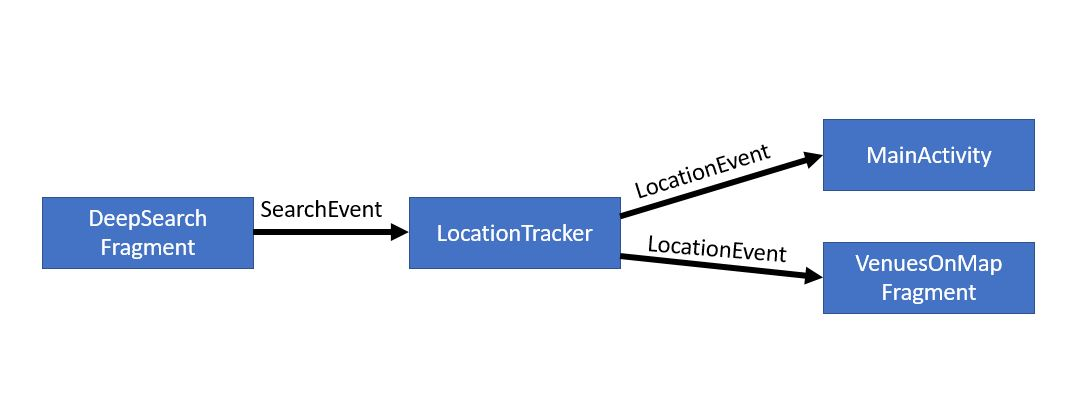
\includegraphics[width=0.8\textwidth]{images/eventBus.jpg}
	\centering
	\caption[]{\textit{EventBus} graph, schematically shows who sends which event type and who receives it}
	\label{fig:eventbus}
\end{figure} 


\begin{itemize}
\item The \textit{LocationTracker} subscribes on it to receive the \textit{SearchEvent}, which tells it to change the accuracy
\item The \textit{SearchEvent} is posted by the \textit{DeepSearchFragement} everytime its view is created
\item The \textit{LocationTracker} posts a \textit{LocationEvent} on the \textit{EventBus}, which contains the Location and is received by the \textit{MainActivity} and the \textit{VenueOnMapFragment}
\item The \textit{MainActivity} receives the \textit{LocationEvent}, stores it locally and sends it every 10 seconds (parameterized) to the server, to update the users position data
\item The \textit{VenueOnMapFragment} receives the \textit{LocationEvent} to update the location of the user on the map and also the location of his friends if the user is logged in
\end{itemize}

\subsection{The Map}
The map is used as a function to show the user graphically where he and his nearby friends are and also the searched venues. The functionality of the map in inside the \textit{VenuesOnMapFragment}, which is part of the \textit{MainActivity}. The map itself is provided by \textit{GoogleMaps}.

There are three different kinds of markers shown on the map. If the user clicks on any marker, a button shows up, which allows him to change to \textit{GoogleMaps} and gets the route to the chosen marker. 

\subsubsection{Marker: Venue}
The venue markers locate the search results on the map. They differ in color, depending on the rating of the venue. Those colors are with the following more or less obvious order:

\begin{itemize}
\item \textbf{grey}: No rating available / no rating yet
\item \textbf{red}: rating between 0 and 1
\item \textbf{orange}: rating between 1 and 2
\item \textbf{yellow}: rating between 2 and 3
\item \textbf{lime}: rating between 3 and 4
\item \textbf{green}: rating between 4 and 5
\end{itemize}

If the user clicks on one of the markers an infoWindow shows up, which shows on image and tells the name, the exact rating and if it is open right now or not. With a click on the infoWindow the user is redirected to the \textit{VenueDetails}, where he can find more additional information about the venue.

\subsection{Marker: Friend}
The friend markers locate the friends of the user, if he is logged in and has nearby friends. The marker of the friends is similar to the marker of the user, except it is green.
The position of his nearby friends are updated everytime, the location of the user changes. 

If the user clicks on on of his friends marker, an \textit{infoWindow} shows up with the avatar and name and if given, also the city and age. With a click on the \textit{infoWindow} the user gets to the profile of his friend.

\subsection{Marker: User}
The user marker locate the user on the map. If the user clicks on himself, a \textit{infoWindow} shows up. If the user is not logged in, it shows the default \textit{infoWindow} with the default avatar. If the user is logged in, it shows his own avatar and additonal info. 

If he clicks on the \textit{infoWindow} he is redirected to his own profile.

 



